% The Loop Economy: a 5-minute lightning talk, Devcon 8, Mumbai, 6 November 2026
% (Lightning Stage, 11:00-11:07). Build: make   (pdflatex, two passes)
% Script and timing: talk.md. Figures are TikZ, inline, so the deck is one file.
\documentclass[aspectratio=169,11pt]{beamer}
\usepackage[T1]{fontenc}
\usepackage{lmodern}
\usepackage{tgheros}
\renewcommand{\familydefault}{\sfdefault}
\usepackage{amsmath,amssymb}
\usepackage{booktabs}
\usepackage{array}
\usepackage{qrcode}
\usepackage{tikz}
\usetikzlibrary{arrows.meta,positioning,calc,fit,backgrounds,decorations.pathreplacing}

% --- one accent, one highlight, thin lines (as docs/talk/slides/figstyle.tex) ---
\definecolor{ink}{RGB}{34,34,34}
\definecolor{soft}{RGB}{105,105,105}
\definecolor{faint}{RGB}{222,222,222}
\definecolor{accent}{RGB}{0,95,115}
\definecolor{accentlight}{RGB}{214,232,236}
\definecolor{warn}{RGB}{196,84,40}
\definecolor{warnlight}{RGB}{247,226,216}
\tikzset{
  every picture/.style={color=ink, line width=0.5pt, font=\small},
  box/.style={draw=ink, rounded corners=2pt, fill=white, inner sep=4pt, minimum height=7mm, align=center},
  maker/.style={box, minimum width=17mm, font=\small\bfseries},
  cat/.style={box, inner sep=2.5pt, minimum height=5mm, font=\scriptsize},
  root/.style={box, fill=accentlight, draw=accent},
  bad/.style={box, fill=warnlight, draw=warn},
  flow/.style={-{Stealth[length=5pt,width=4pt]}, line width=0.6pt},
  sub/.style={-{Stealth[length=4pt,width=3.5pt]}, line width=0.5pt, color=soft},
  strong/.style={flow, color=accent, line width=0.9pt},
  lbl/.style={font=\footnotesize, text=ink, inner sep=1.5pt, fill=white},
  note/.style={font=\footnotesize, text=soft, align=center},
  rate/.style={font=\footnotesize, text=accent, inner sep=1pt, fill=white},
  person/.style={circle, draw=ink, fill=white, minimum size=5mm, inner sep=0pt},
}

% --- a quiet theme ----------------------------------------------------------
\usetheme{default}
\setbeamertemplate{navigation symbols}{}
\setbeamercolor{normal text}{fg=ink}
\setbeamercolor{structure}{fg=accent}
\setbeamercolor{frametitle}{fg=ink}
\setbeamercolor{alerted text}{fg=warn}
\setbeamerfont{frametitle}{size=\Large, series=\bfseries}
\setbeamertemplate{frametitle}{\vspace*{5mm}\insertframetitle\par\vspace*{0mm}}
\setbeamertemplate{itemize items}{\textcolor{accent}{\raisebox{0.3ex}{\rule{0.85ex}{0.85ex}}}}
\setbeamertemplate{itemize subitem}{\textcolor{soft}{--}}
\setlength{\leftmargini}{1.2em}
\setbeamersize{text margin left=10mm, text margin right=10mm}
% Every slide carries the repository and the project's page (devcon.txt;
% Peter, 2026-11-05). A frame inside a group may change either side, or
% add a centre.
\newcommand{\footleft}{github.com/petfold/loopmarket}
\newcommand{\footright}{loopmarket.eth.limo}
\newcommand{\footcentre}{}
\setbeamertemplate{footline}{%
  \leavevmode\hbox to \paperwidth{\hspace*{10mm}%
    \rlap{\footnotesize\color{soft}\footleft}\hfill
    {\footnotesize\color{ink}\footcentre}\hfill
    \llap{\footnotesize\color{soft}\footright\hspace{6mm}\insertframenumber}\hspace*{10mm}}%
  \vspace*{3.5mm}}

\newcommand{\sep}{\enspace\textperiodcentered\enspace}
\newcommand{\tick}{\textcolor{accent}{\checkmark}}
\newcommand{\todo}{\textcolor{soft}{$\circ$}}
\newcommand{\code}[1]{{\ttfamily #1}}
\newcommand{\qr}[2]{\qrcode[height=#1]{#2}}
\newcommand{\shade}[3]{\fcolorbox{#1}{#1}{\parbox{#2}{\raggedright #3}}}

\title{The Loop Economy}
\subtitle{A universal combinatorial marketplace\\ without a platform}
\author{Peter F\"oldi\'ak}
\date{Devcon 8\sep Mumbai\sep 6 November 2026}

\begin{document}

% ================================================================ 1 title
{\renewcommand{\footleft}{}
\begin{frame}
  \vspace*{6mm}
  \begin{columns}[c]
    \begin{column}{0.66\textwidth}
      {\fontsize{28}{32}\selectfont\bfseries\inserttitle\par}
      \vspace{3mm}
      {\large\insertsubtitle\par}
      \vspace{10mm}
      {\normalsize\insertauthor\quad{\color{accent}@petfold}\par}
      \vspace{1.5mm}
      {\small\color{soft}\insertdate\par}
      \vspace{8mm}
      {\footnotesize\color{soft}loopmarket\sep ontodag\sep factbond\sep on Swarm\par}
    \end{column}
    \begin{column}{0.30\textwidth}
      \centering
      \qr{31mm}{https://github.com/petfold/loopmarket}\par
      \vspace{2mm}
      {\footnotesize github.com/petfold/loopmarket\par}
    \end{column}
  \end{columns}
\end{frame}
}

% ================================================================ 2 problem
\begin{frame}{Most good trades never happen}
  \begin{columns}[c]
    \begin{column}{0.50\textwidth}
      \small
      \begin{itemize}\setlength{\itemsep}{2mm}
        \item Markets let strangers cooperate, voluntarily: a part of individual freedom.
        \item Online, that means \textbf{search}: shop after shop, each with its own catalogue, terms and checkout, and you never know you found the best deal.
        \item Or a \textbf{platform} that owns the index: it takes a cut, decides who is seen, and can delist anyone.
      \end{itemize}
      \vspace{3mm}
      {\color{accent}\bfseries Most mutually profitable trades fail on discovery, not on price: finding them costs more than they are worth.\par}
    \end{column}
    \begin{column}{0.48\textwidth}
      \centering
      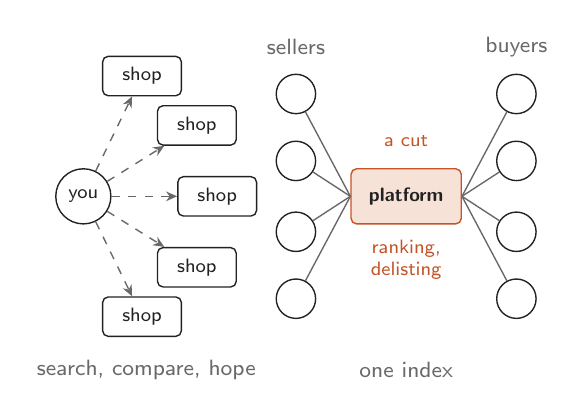
\begin{tikzpicture}[shop/.style={box, minimum width=10mm, minimum height=5mm, inner sep=1.5pt, font=\scriptsize}]
        % search: one buyer, many islands
        \node[person, minimum size=7mm, font=\scriptsize] (you) at (0,0) {you};
        \foreach \i/\a in {1/64,2/32,3/0,4/-32,5/-64} {
          \node[shop] (s\i) at (\a:17mm) {shop};
          \draw[sub, dashed] (you) -- (s\i);
        }
        \node[note] at (8mm,-22mm) {search, compare, hope};
        % platform: everyone through one company
        \begin{scope}[xshift=41mm]
          \node[bad, minimum width=14mm, font=\scriptsize\bfseries] (P) at (0,0) {platform};
          \foreach \i/\y in {1/13,2/4.5,3/-4.5,4/-13} {
            \node[person] (m\i) at (-14mm,\y mm) {};
            \node[person] (b\i) at (14mm,\y mm) {};
            \draw[soft] (m\i) -- (P.west); \draw[soft] (P.east) -- (b\i);
          }
          \node[font=\scriptsize, text=warn] at (0,7mm) {a cut};
          \node[font=\scriptsize, text=warn, align=center] at (0,-8mm) {ranking,\\ delisting};
          \node[note] at (-14mm,19mm) {sellers}; \node[note] at (14mm,19mm) {buyers}; \node[note] at (0,-22mm) {one index};
        \end{scope}
      \end{tikzpicture}
    \end{column}
  \end{columns}
\end{frame}

% ================================================================ 3 idea
\begin{frame}{Describe, don't search: solvers find the trade}
  \vspace{-2mm}
  \begin{columns}[T]
    \begin{column}{0.31\textwidth}
      \centering
      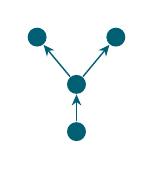
\begin{tikzpicture}[d/.style={circle, fill=accent, inner sep=0pt, minimum size=2.4mm}]
        \node[d] (a) at (-5mm,6mm) {}; \node[d] (b) at (5mm,6mm) {};
        \node[d] (c) at (0,0) {}; \node[d] (e) at (0,-6mm) {};
        \draw[sub, color=accent] (c) -- (a); \draw[sub, color=accent] (c) -- (b);
        \draw[sub, color=accent] (e) -- (c);
      \end{tikzpicture}\par
      \vspace{1.5mm}
      {\large\bfseries\color{accent}universal\par}\vspace{0.5mm}
    \end{column}
    \begin{column}{0.31\textwidth}
      \centering
      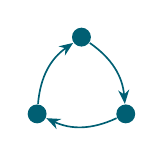
\begin{tikzpicture}[d/.style={circle, fill=accent, inner sep=0pt, minimum size=2.4mm}]
        \node[d] (a) at (90:6.5mm) {}; \node[d] (b) at (210:6.5mm) {}; \node[d] (c) at (330:6.5mm) {};
        \draw[flow, color=accent] (a) to[bend left=25] (c);
        \draw[flow, color=accent] (c) to[bend left=25] (b);
        \draw[flow, color=accent] (b) to[bend left=25] (a);
      \end{tikzpicture}\par
      \vspace{1.5mm}
      {\large\bfseries\color{accent}combinatorial\par}\vspace{0.5mm}
    \end{column}
    \begin{column}{0.31\textwidth}
      \centering
      
\begin{tikzpicture}[d/.style={circle, fill=accent, inner sep=0pt, minimum size=2.4mm}]
        \foreach \i in {0,...,5} { \node[d] (p\i) at (\i*60:7mm) {}; }
        \foreach \i/\j in {0/1,1/2,2/3,3/4,4/5,5/0,0/2,1/4,3/5} { \draw[color=accent] (p\i) -- (p\j); }
      \end{tikzpicture}\par
      \vspace{1.5mm}
      {\large\bfseries\color{accent}permissionless\par}\vspace{0.5mm}
    \end{column}
  \end{columns}
  \vspace{1mm}
  \begin{columns}[T]\small
    \begin{column}{0.31\textwidth}
      Anything that can be described exactly: rides, repairs, parcels, storage, energy, care\dots\ and money, as one more offer. Not only tokens.
    \end{column}
    \begin{column}{0.31\textwidth}
      Many offers combine into one trade: loops of three, five, ten makers; a courier's leg composed into a delivery. Algorithms do the searching.
    \end{column}
    \begin{column}{0.31\textwidth}
      Every maker keeps their own offer book on Swarm. No platform, no protocol fee, nobody who can delist you.
    \end{column}
  \end{columns}
  \vspace{4mm}
  \begin{center}
    \shade{accentlight}{0.95\textwidth}{\centering\small
      CoW Protocol finds coincidences of wants among tokens, to beat the AMM price.\\
      \textbf{loopmarket finds them where there is no AMM to beat.}}
  \end{center}
\end{frame}

% ================================================================ 4 offer
\begin{frame}{One offer form for everything}
  \vspace{-1mm}
  \centering
  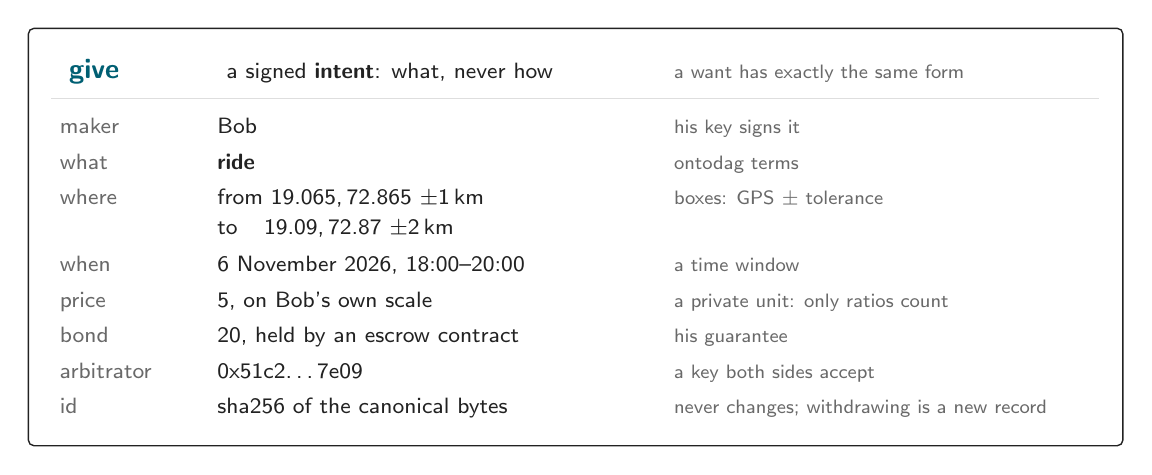
\begin{tikzpicture}[k/.style={anchor=base west, font=\footnotesize, text=soft, inner sep=0pt},
                      v/.style={anchor=base west, font=\footnotesize, inner sep=0pt},
                      c/.style={anchor=base west, font=\scriptsize, text=soft, inner sep=0pt}]
    \node[box, minimum width=139mm, minimum height=53mm, anchor=north west] at (0,0) {};
    \node[anchor=base west, font=\normalsize\bfseries, text=accent] at (4mm,-6.5mm) {give};
    \node[anchor=base west, font=\footnotesize] at (24mm,-6.5mm) {a signed \textbf{intent}: what, never how};
    \node[c] at (82mm,-6.5mm) {a want has exactly the same form};
    \draw[faint] (3mm,-9mm) -- (136mm,-9mm);
    \foreach \y/\key/\val/\com in {
        -13.5/maker/{Bob}/{his key signs it},
        -18/what/{\textbf{ride}}/{ontodag terms},
        -22.5/where/{from 19.065,\,72.865 $\pm$1\,km}/{boxes: GPS $\pm$ tolerance},
        -26.3/{}/{to\phantom{m} 19.09,\,72.87 $\pm$2\,km}/{},
        -31/when/{6 November 2026, 18:00--20:00}/{a time window},
        -35.5/price/{5, on Bob's own scale}/{a private unit: only ratios count},
        -40/bond/{20, held by an escrow contract}/{his guarantee},
        -44.5/arbitrator/{0x51c2\dots7e09}/{a key both sides accept},
        -49/id/{sha256 of the canonical bytes}/{never changes; withdrawing is a new record}} {
      \node[k] at (4mm,\y mm) {\key};
      \node[v] at (24mm,\y mm) {\val};
      \node[c] at (82mm,\y mm) {\com};
    }
  \end{tikzpicture}\par
  \vspace{2.5mm}
  \raggedright
  {\small Own scale: $k$ gives and $m$ wants need $k+m$ prices, not $k\times m$ exchange rates.\par}
  \vspace{1mm}
  {\scriptsize\ttfamily\color{soft}\$ loop give ride \textquotesingle{}from(Jio)\textquotesingle{} \textquotesingle{}to(BOM)\textquotesingle{} \textquotesingle{}time(2026-11-06T12:30:00Z..2026-11-06T14:30:00Z)\textquotesingle{} 5\par}
\end{frame}

% ================================================================ 5 loops
\begin{frame}{Loops: the trade nobody could find}
  \vspace{-1mm}
  \begin{columns}[T]
    \begin{column}{0.42\textwidth}
      \centering
      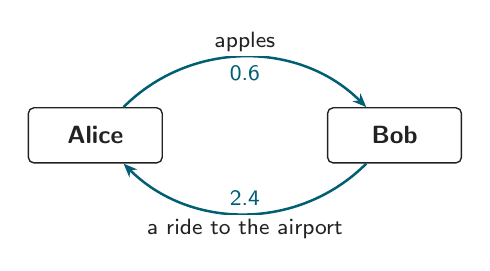
\begin{tikzpicture}
        \node[maker] (A) at (0,0) {Alice};
        \node[maker] (B) at (38mm,0) {Bob};
        \draw[strong] (A) to[bend left=45] node[lbl, above] {apples} node[rate, below=0.6mm] {0.6} (B);
        \draw[strong] (B) to[bend left=45] node[lbl, below] {a ride to the airport} node[rate, above=0.6mm] {2.4} (A);
      \end{tikzpicture}\par
      \vspace{1.5mm}
      {\small\color{accent}$\prod r = 0.6\times 2.4 = 1.44 > 1$\par}
      \vspace{1mm}
      {\small Barter needs a \emph{double coincidence of wants}, which is rare.\par}
    \end{column}
    \begin{column}{0.54\textwidth}
      \centering
      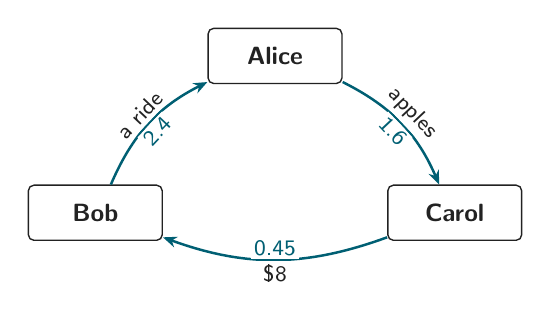
\begin{tikzpicture}
        \node[maker] (A) at (90:12.5mm) {Alice};
        \node[maker] (C) at (-18:24mm) {Carol};
        \node[maker] (B) at (198:24mm) {Bob};
        \draw[strong] (A) to[bend left=20] node[lbl, sloped, above] {apples} node[rate, sloped, below] {1.6} (C);
        \draw[strong] (C) to[bend left=20] node[lbl, below] {\$8} node[rate, above] {0.45} (B);
        \draw[strong] (B) to[bend left=20] node[lbl, sloped, above] {a ride} node[rate, sloped, below] {2.4} (A);
      \end{tikzpicture}\par
      \vspace{1mm}
      {\small\color{accent}$\prod r = 1.6\times 0.45\times 2.4 = 1.728 > 1$\par}
      \vspace{1mm}
      {\small Bob wants money, not apples. No pair can trade, yet the loop clears: money is one more leg.\par}
    \end{column}
  \end{columns}
  \vspace{2mm}
  \shade{accentlight}{0.975\textwidth}{\small
    A leg's rate $r$ is the wanter's price over the giver's, each on their own scale. $\prod r>1$ is a \textbf{negative cycle} under $-\log r$: Bellman--Ford finds it, as in DEX arbitrage, and the makers keep the surplus.}
\end{frame}

% ================================================================ 6 ontodag
{\renewcommand{\footleft}{github.com/petfold/ontodag}\renewcommand{\footright}{ontodag.eth.limo}
\begin{frame}{OntoDAG: one relation, \emph{fits within}}
  \vspace{-1mm}
  \begin{columns}[T]
    \begin{column}{0.55\textwidth}
      \centering
      % edges from ontodag's core pack v14 (a selection); arrows point to the supercategory
      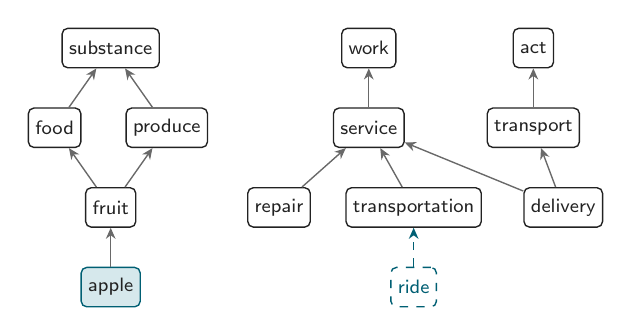
\begin{tikzpicture}[x=0.95mm, y=0.92mm]
        \node[cat] (substance) at (7.5,33) {substance};
        \node[cat] (work) at (42,33) {work};
        \node[cat] (act) at (64,33) {act};
        \node[cat] (food) at (0,22) {food};
        \node[cat] (produce) at (15,22) {produce};
        \node[cat] (service) at (42,22) {service};
        \node[cat] (transport) at (64,22) {transport};
        \node[cat] (fruit) at (7.5,11) {fruit};
        \node[cat] (repair) at (30,11) {repair};
        \node[cat] (transportation) at (48,11) {transportation};
        \node[cat] (delivery) at (68,11) {delivery};
        \node[cat, fill=accentlight, draw=accent] (apple) at (7.5,0) {apple};
        \node[cat, draw=accent, dashed, text=accent] (ride) at (48,0) {ride};
        \foreach \a/\b in {food/substance, produce/substance, fruit/food, fruit/produce, apple/fruit,
                           service/work, transport/act, repair/service, transportation/service,
                           delivery/service, delivery/transport} { \draw[sub] (\a) -- (\b); }
        \draw[sub, color=accent, dashed] (ride) -- (transportation);
      \end{tikzpicture}\par
      \vspace{1mm}
      {\tiny\color{soft}edges from ontodag's core pack (a selection); \textcolor{accent}{ride} is added with \code{put}\par}
      \vspace{2.5mm}
      \raggedright
      {\scriptsize\ttfamily
        \textcolor{soft}{\$} odag put ride transportation\\[0.4mm]
        \textcolor{soft}{\$} odag get food produce\\[0.4mm]
        almond apple apricot artichoke \dots\ {\rmfamily\color{soft}(117 items)}\par}
    \end{column}
    \begin{column}{0.43\textwidth}
      \small
      \begin{itemize}\setlength{\itemsep}{1.2mm}
        \item \textbf{A DAG, not a tree}: an apple is food \emph{and} produce. No folder to choose.
        \item \textbf{Space and time too}: \code{geo(19.06,72.86±1km)}, \code{time(2026-11-06)}, ordered by computation, never stored.
        \item \textbf{Canonical}: equal content, equal root hash. Offers pin it; packs live on Swarm.
        \item \textbf{A shared core}: about 4,800 categories, by consensus over WordNet, SUMO, Wikidata, schema.org\dots
      \end{itemize}
    \end{column}
  \end{columns}
  \vspace{1mm}
  {\small\color{accent}\bfseries A give matches a want when it fits within it: in meaning, in place and in time.\par}
\end{frame}
}

% ================================================================ 7 swarm
\begin{frame}{Swarm: a server nobody owns}
  \vspace{-1mm}
  \footnotesize
  \renewcommand{\arraystretch}{1.2}
  \begin{tabular}{@{}>{\raggedright\arraybackslash}p{57mm}>{\raggedright\arraybackslash}p{78.5mm}@{}}
    \toprule
    \textbf{\color{accent}what Swarm gives} & \textbf{\color{accent}what loopmarket does with it} \\
    \midrule
    \textbf{Content addressing}: data is named by its hash
      & an offer's id is its hash; equal books give equal roots, byte for byte; inclusion proofs are checked on chain \\
    \textbf{Feeds}: mutable pointers, signed by their owner
      & each maker's book is their own feed: identity is a key; no account, no platform \\
    \textbf{Postage}: storage prepaid, no hosting account; it all goes to the node operators
      & a maker pays only for their own book, and reading it costs them nothing \\
    \textbf{Thousands of independent nodes}, permissionless
      & nobody can delist an offer; an aggregator that drops a book is caught by an absence proof \\
    \textbf{Encryption and access control}, client side
      & delivery details are sealed to the counterparty, inside the book \\
    \textbf{Websites are content too}
      & the market page is itself a Swarm site: it folds every book in the browser \\
    \bottomrule
  \end{tabular}
  \vspace{2.5mm}

  On chain only what needs consensus: one announcement per book, the batches, the escrow.
\end{frame}

% ================================================================ 8 lifecycle
\begin{frame}{From offer to delivery}
  \centering
  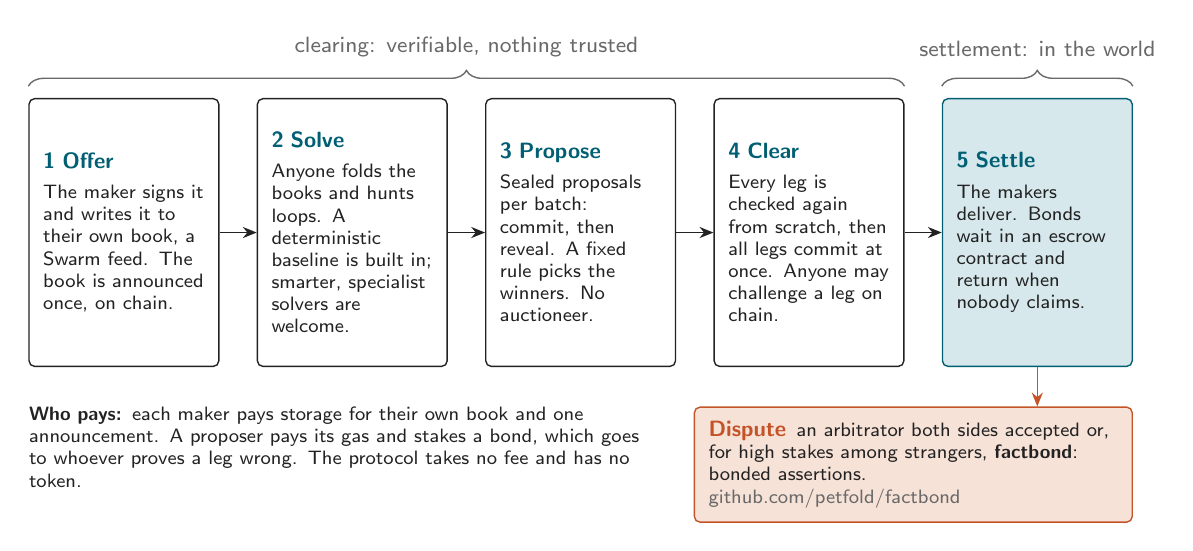
\begin{tikzpicture}[x=1mm, y=1mm,
      nohyph/.style={execute at begin node={\hyphenpenalty=10000\exhyphenpenalty=10000\rightskip=0pt plus 1fil}},
      stage/.style={box, nohyph, text width=20.5mm, minimum height=34mm, align=left, anchor=north, inner sep=1.8mm, font=\scriptsize}]
    \node[stage] (s1) at (0,0)   {{\footnotesize\bfseries\color{accent}1 Offer}\\[1mm]The maker signs it and writes it to their own book, a Swarm feed. The book is announced once, on chain.};
    \node[stage] (s2) at (29,0)  {{\footnotesize\bfseries\color{accent}2 Solve}\\[1mm]Anyone folds the books and hunts loops. A deterministic baseline is built in; smarter, specialist solvers are welcome.};
    \node[stage] (s3) at (58,0)  {{\footnotesize\bfseries\color{accent}3 Propose}\\[1mm]Sealed proposals per batch: commit, then reveal. A fixed rule picks the winners. No auctioneer.};
    \node[stage] (s4) at (87,0)  {{\footnotesize\bfseries\color{accent}4 Clear}\\[1mm]Every leg is checked again from scratch, then all legs commit at once. Anyone may challenge a leg on chain.};
    \node[stage, fill=accentlight, draw=accent] (s5) at (116,0) {{\footnotesize\bfseries\color{accent}5 Settle}\\[1mm]The makers deliver. Bonds wait in an escrow contract and return when nobody claims.};
    \foreach \a/\b in {s1/s2, s2/s3, s3/s4, s4/s5} { \draw[flow] (\a.east) -- (\b.west); }
    \draw[decorate, decoration={brace, amplitude=2mm}, soft] ($(s1.north west)+(0,1.5)$) -- node[note, above=2.5mm] {clearing: verifiable, nothing trusted} ($(s4.north east)+(0,1.5)$);
    \draw[decorate, decoration={brace, amplitude=2mm}, soft] ($(s5.north west)+(0,1.5)$) -- node[note, above=2.5mm] {settlement: in the world} ($(s5.north east)+(0,1.5)$);
    \node[bad, nohyph, text width=52mm, align=left, font=\scriptsize, anchor=north east, inner sep=1.8mm] (d) at ($(s5.south east)+(0,-5)$)
      {{\footnotesize\bfseries\color{warn}Dispute}\enspace an arbitrator both sides accepted or, for high stakes among strangers, \textbf{factbond}: bonded assertions.\\ {\color{soft}github.com/petfold/factbond}};
    \draw[flow, color=warn] (s5.south) -- (s5.south |- d.north);
    \node[nohyph, anchor=north west, text width=80mm, align=left, font=\scriptsize, inner sep=0pt] at ($(s1.south west)+(0,-5)$)
      {\textbf{Who pays:} each maker pays storage for their own book and one announcement. A proposer pays its gas and stakes a bond, which goes to whoever proves a leg wrong. The protocol takes no fee and has no token.};
  \end{tikzpicture}
\end{frame}

% ================================================================ 9 status
{\renewcommand{\footcentre}{\bfseries @petfold}
\begin{frame}{Where it stands: open source, live at test amounts}
  \vspace{-1mm}
  \begin{columns}[T]
    \begin{column}{0.26\textwidth}
      {\small\bfseries\color{accent}loopmarket\par}
      {\scriptsize\color{soft}Python, BSD-3, on PyPI\par}
      \vspace{1.5mm}
      \scriptsize
      \tick\ offers, books on Swarm, the fold, the baseline solver, clearing\\[0.8mm]
      \tick\ on Gnosis: announcements, sealed batches, challengeable clearing, escrow\\[0.8mm]
      \tick\ the \code{loop} command line; the market in a browser\\[0.8mm]
      \todo\ next: paying solvers, privacy, first real users
    \end{column}
    \begin{column}{0.24\textwidth}
      {\small\bfseries\color{accent}ontodag\par}
      {\scriptsize\color{soft}Python, BSD-3, on PyPI\par}
      \vspace{1.5mm}
      \scriptsize
      \tick\ the DAG store, typed values (time, geo, mass, \dots), canonical roots, verifiable answers\\[0.8mm]
      \tick\ core: about 4,800 categories, plus ten domain packs, also on Swarm
    \end{column}
    \begin{column}{0.20\textwidth}
      {\small\bfseries\color{accent}factbond\par}
      {\scriptsize\color{soft}bonded assertions\par}
      \vspace{1.5mm}
      \scriptsize
      \tick\ the assertion contract on Gnosis, the escrow's resolver\\[0.8mm]
      \todo\ next: the scored simulation that gates real stakes
    \end{column}
    \begin{column}{0.24\textwidth}
      \centering
      \qr{23mm}{https://github.com/petfold/loopmarket}\par
      {\tiny github.com/petfold/loopmarket\par}
      \vspace{2mm}
      \qr{16mm}{https://github.com/petfold/ontodag}\par
      {\tiny github.com/petfold/ontodag\par}
    \end{column}
  \end{columns}
  \vspace{3mm}
  \shade{warnlight}{0.975\textwidth}{\small
    \textbf{What stays hard:} oracles for physical delivery\sep private matching (ZK fits-within proofs)\sep wash loops\sep capture of the catalogue\sep books thick enough to close loops}
\end{frame}
}

% ================================================================ backup
\appendix
\begin{frame}{Backup: one want, many gives}
  \centering
  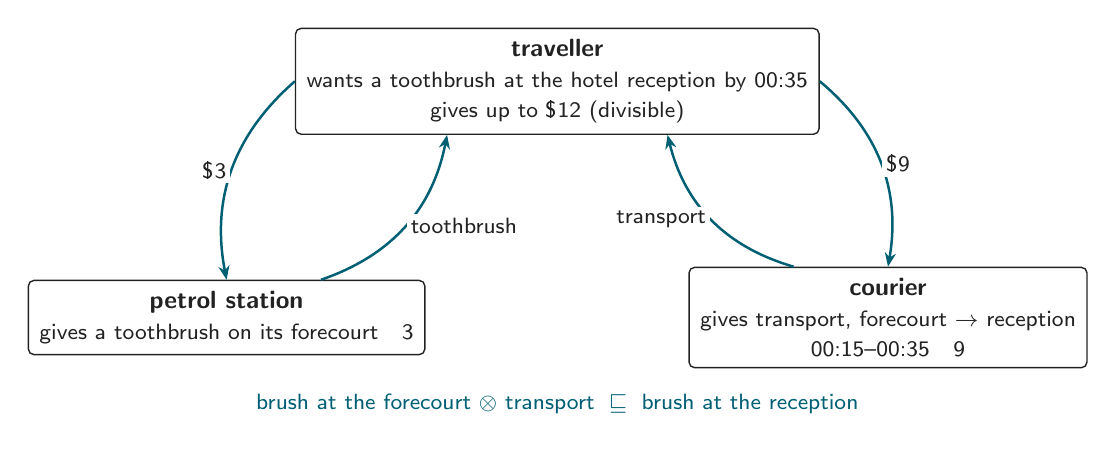
\begin{tikzpicture}
    \node[maker, align=center, font=\small\bfseries] (T) at (0,0) {traveller\\{\footnotesize\mdseries wants a toothbrush at the hotel reception by 00:35}\\{\footnotesize\mdseries gives up to \$12 (divisible)}};
    \node[maker, align=center, font=\small\bfseries] (S) at (-42mm,-30mm) {petrol station\\{\footnotesize\mdseries gives a toothbrush on its forecourt\quad 3}};
    \node[maker, align=center, font=\small\bfseries] (C) at (42mm,-30mm) {courier\\{\footnotesize\mdseries gives transport, forecourt $\to$ reception}\\{\footnotesize\mdseries 00:15--00:35\quad 9}};
    \draw[strong] (T.west) to[bend right=30] node[lbl, left] {\$3} (S.north);
    \draw[strong] (T.east) to[bend left=30] node[lbl, right] {\$9} (C.north);
    \draw[strong] ($(S.north)+(12mm,0)$) to[bend right=30] node[lbl, right] {toothbrush} ($(T.south)+(-14mm,0)$);
    \draw[strong] ($(C.north)+(-12mm,0)$) to[bend left=30] node[lbl, left] {transport} ($(T.south)+(14mm,0)$);
    \node[note, text=accent] at (0,-41mm) {brush at the forecourt $\otimes$ transport $\;\sqsubseteq\;$ brush at the reception};
  \end{tikzpicture}\par
  \vspace{3mm}
  \raggedright
  {\small Every give names one plain thing: the courier sells carriage, not toothbrushes. The \emph{one} want holds the conjunction, so it clears all or nothing, and one payment splits \$3\,+\,\$9.\par}
\end{frame}

\begin{frame}{Backup: why a personal scale}
  \centering
  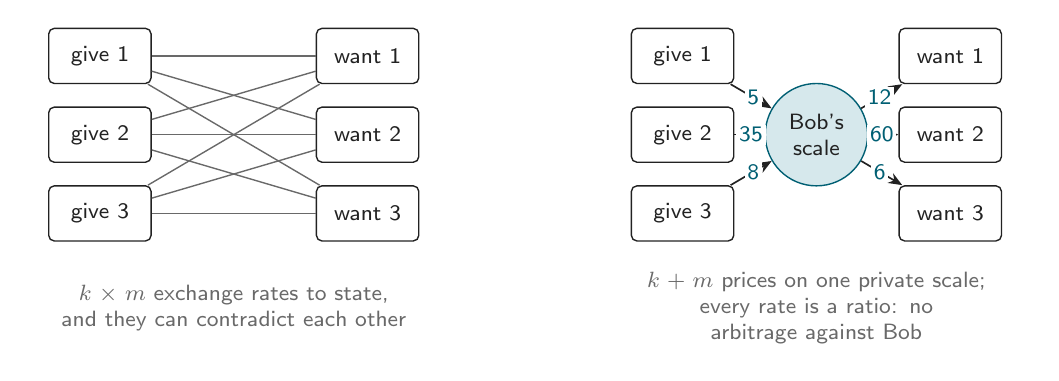
\begin{tikzpicture}[item/.style={box, inner sep=2.5pt, minimum width=13mm, font=\footnotesize}]
    \begin{scope}
      \foreach \i/\y in {1/10,2/0,3/-10} { \node[item] (g\i) at (0,\y mm) {give \i}; }
      \foreach \j/\y in {1/10,2/0,3/-10} { \node[item] (w\j) at (34mm,\y mm) {want \j}; }
      \foreach \i in {1,2,3} \foreach \j in {1,2,3} { \draw[soft] (g\i) -- (w\j); }
      \node[note, text width=50mm] at (17mm,-22mm) {$k \times m$ exchange rates to state,\\ and they can contradict each other};
    \end{scope}
    \begin{scope}[xshift=74mm]
      \node[root, circle, inner sep=1pt, minimum size=13mm, font=\footnotesize, align=center] (S) at (17mm,0) {Bob's\\ scale};
      \foreach \i/\y/\p in {1/10/5,2/0/35,3/-10/8} { \node[item] (g\i) at (0,\y mm) {give \i}; \draw[flow] (g\i) -- node[rate, pos=0.55] {\p} (S); }
      \foreach \j/\y/\p in {1/10/12,2/0/60,3/-10/6} { \node[item] (w\j) at (34mm,\y mm) {want \j}; \draw[flow] (S) -- node[rate, pos=0.45] {\p} (w\j); }
      \node[note, text width=52mm] at (17mm,-22mm) {$k + m$ prices on one private scale;\\ every rate is a ratio: no arbitrage against Bob};
    \end{scope}
  \end{tikzpicture}\par
  \vspace{5mm}
  \raggedright
  {\small The scale is bookkeeping, a personal numeraire: nothing is issued, held or transferred. Only ratios leave the maker, and round a loop the scales cancel. A batch is scored by the sum of the logs of its loops' surplus factors, so no common unit is ever needed.\par}
\end{frame}

\begin{frame}{Backup: CoW Protocol and loopmarket}
  \vspace{-1mm}
  \footnotesize
  \renewcommand{\arraystretch}{1.0}
  \begin{tabular}{@{}>{\raggedright\arraybackslash}p{22mm}>{\raggedright\arraybackslash}p{50mm}>{\raggedright\arraybackslash}p{59mm}@{}}
    \toprule
    & \textbf{CoW Protocol} & \textbf{loopmarket} \\
    \midrule
    traded & tokens & anything the catalogue describes, money included \\
    matching & the same two token addresses, a limit price & fits within, in the catalogue: meaning, place, time \\
    unit of price & token amounts, scored in the native token & each maker's own scale; scored in logs, unit-free \\
    intents live in & CoW's order book & each maker's book, a Swarm feed \\
    auctioneer & the autopilot, one per chain & none: sealed batches on chain, a rule anyone recomputes \\
    solvers & bonded and allowlisted & anyone who posts the bond \\
    after the trade & nothing: the tokens arrived & delivery, bonds in escrow, arbitration \\
    \bottomrule
  \end{tabular}
  \vspace{2mm}

  {\small Same family: signed intents, batches, solvers trusted with nothing. Different market: CoW's rings compete with an AMM price, a loop of rides and repairs with no trade at all. The fairness filter is CoW's CIP-67, generalised to cycles.\par}
\end{frame}

\begin{frame}{Backup: who pays for what}
  \small
  \renewcommand{\arraystretch}{1.35}
  \begin{tabular}{@{}>{\raggedright\arraybackslash}p{22mm}>{\raggedright\arraybackslash}p{59mm}>{\raggedright\arraybackslash}p{50mm}@{}}
    \toprule
    & \textbf{pays} & \textbf{gets} \\
    \midrule
    maker & storage for their own book; one announcement & the trade, at or better than their own price \\
    solver & the gas to post a proposal, and a bond & designed: a spread leg inside the loop it found \\
    challenger & gas & the bond of a proposal it proves wrong \\
    aggregator & its own storage and bandwidth & paid serving, never paid inclusion \\
    the protocol & \multicolumn{2}{>{\raggedright\arraybackslash}p{113mm}@{}}{\textbf{nothing, either way}: no fee, no token, no rewards. A real loop looks exactly like a wash trade, so any reward tied to volume would pay people to trade with themselves.} \\
    \bottomrule
  \end{tabular}
\end{frame}

\end{document}
